\section{Křižovatka}\label{sec:krizovatka}

Shrnutí hledání na grafu, definice grafu.

Popis různých vzhledů křižovatky.
Převod křižovatky na graf a parametry převodu.

%
%Existuje řada algoritmů řešících problém plánování více agentů, které jsou založeny na prohledávání orientovaného grafu.
%Z tohoto důvodu je nutné nejdříve převést křižovatku na graf.
%Převod je proveden rozdělením křižovatky na~diskrétní nepřekrývající~se bloky zaplňující celou plochu,
%kde auta mohou mezi sousedními bloky přejíždět.
%
%Formálně je křižovatka převedena na orientovaný graf,
%kde~každý blok je reprezentován jedním vrcholem a hrany vedou mezi sousedními bloky.
%%Vzdálenost mezi sousedními bloky (čas přejezdu) je u~všech bloků stejný a trvá právě jeden krok simulace.  TODO
%
%Bloky jsou rozděleny do~třech skupin.
%První skupina jsou vrcholy reprezentující vnitřní \emph{plochu} křižovatky.
%Zbylé dvě skupiny reprezentují \emph{vjezdy} do~křižovatky a \emph{výjezdy} z~křižovatky.
%\emph{Vjezdy} jsou vrcholy, ze~kterých vede pouze jedna hrana a žádná hrana do~nich nevede.
%Obdobně vrcholy výjezdů naopak nemají žádné hrany vedoucí z~nich a právě jednu hranu směřující do~nich.
%
%Simulátor nabízí $3$~možné \emph{typy} křižovatek určené rozdělením plochy na bloky.
%Tyto~\emph{typy} budu nazývat \emph{Čtvercové} (Sekce~\ref{subsec:ctvercovy_typ}), \emph{Oktagonální} (Sekce~\ref{subsec:oktagonalni_typ})
%a~\emph{Hexagonální} (Sekce~\ref{subsec:hexagonalni_typ}).
%
%Rozdělení křižovatky má určité parametry ovlivňující výsledný graf.
%Těmito parametry jsou \emph{granularita}, \emph{vjezdy} a~\emph{výjezdy}.
%
%\emph{Granularita} značí na~jak velké množství bloků je křižovatka rozdělena.
%Přesný význam granularity se liší u každého typu a je popsán zvlášť u~každého typu.
%Na~\emph{granularitě} závisí tzv.~\emph{velikost bloku}.
%Tato~velikost značí velikost hlavního bloku (vzdálenost mezi vrcholy), opět se ale u~různých typů liší.
%
%Každý typ křižovatky má předurčený počet \emph{směrů} ze~kterých auta přijíždějí.
%\emph{Vjezdy} značí množství vrcholů reprezentujících pruhy vjezdů z~každého \emph{směru} křižovatky.
%\emph{Výjezdy} mají podobný význam, určují počet výjezdních pruhů z~každého \emph{směru}.
%Jelikož se na silnicích auta pohybují po pravé straně silnice,
%jsou vjezdy a~výjezdy z~jednoho směru seřazeny vůči hraně křižovatky zleva doprava v~pořadí
%\emph{mezeraL}, \emph{výjezdy}, \emph{mezeraS}, \emph{vjezdy}, \emph{mezeraP}.
%Kde~\emph{mezeraL}, \emph{mezeraS} a~\emph{mezeraP} značí posloupnost vrcholů na~hraně křižovatky
%nesousedících s~vjezdem ani~výjezdem.
%Všechny \emph{vjezdy} jsou vždy přímo vedle sebe a \emph{výjezdy} taktéž.
%Většina křižovatek je symetrická proto jsem určil, že velikost \emph{mezeraL} bude shodná s~\emph{mezerouP}.
%Opět kvůli symetričnosti jsem zvolil velikost \emph{mezeryS} co nejblíže velikostei \emph{mezeryL} a~\emph{mezeryP}.
%\emph{MezeraS} je tedy rovna \emph{mezeřeL}, nebo je o~jedna větší.
%
%\subsection{Čtvercový typ}\label{subsec:ctvercovy_typ}
%
%\emph{Čtvercový typ} křižovatky rozděluje plochu do~čtvercových bloků.
%Celková \emph{plocha} křižovatky tvoří (až na~vjezdy a~výjezdy) čtverec.
%
%Granularita značí počet bloků na~jedné straně plochy křižovatky.
%Celkový počet bloků plochy křižovatky tudíž činí $g^2$, kde $g$ je granularita křižovatky.
%Blok je převeden na vrchol s pozicí uprostřed bloku.
%Mezi každými bloky, který spolu sdílí hranu, vede ve výsledným grafu hrana.
%Tento typ křižovatky má čtyři směry, jeden směr na~každé straně čtverce celkové plochy.
%Křižovatka je převedena na~graf s~$g^2 + 4i + 4o$ vrcholy, kde $g$ značí granularitu, $i$~vjezdy a $o$~výjezdy.
%
%Ukázka křižovatky s~granularitou~$4$, jedním vjezdem a jedním výjezdem je vidět na~obrázku~\ref{fig:square_type_graph}.
%Na~obrázku jsou šedou barvou označeny vrcholy značící běžnou plochu křižovatky,
%červeno-šedou barvou označeny vrcholy reprezentující vjezdy a modro-šedé vrcholy reprezentují výjezdy.
%
%\begin{figure}[h]
%	\centering
%	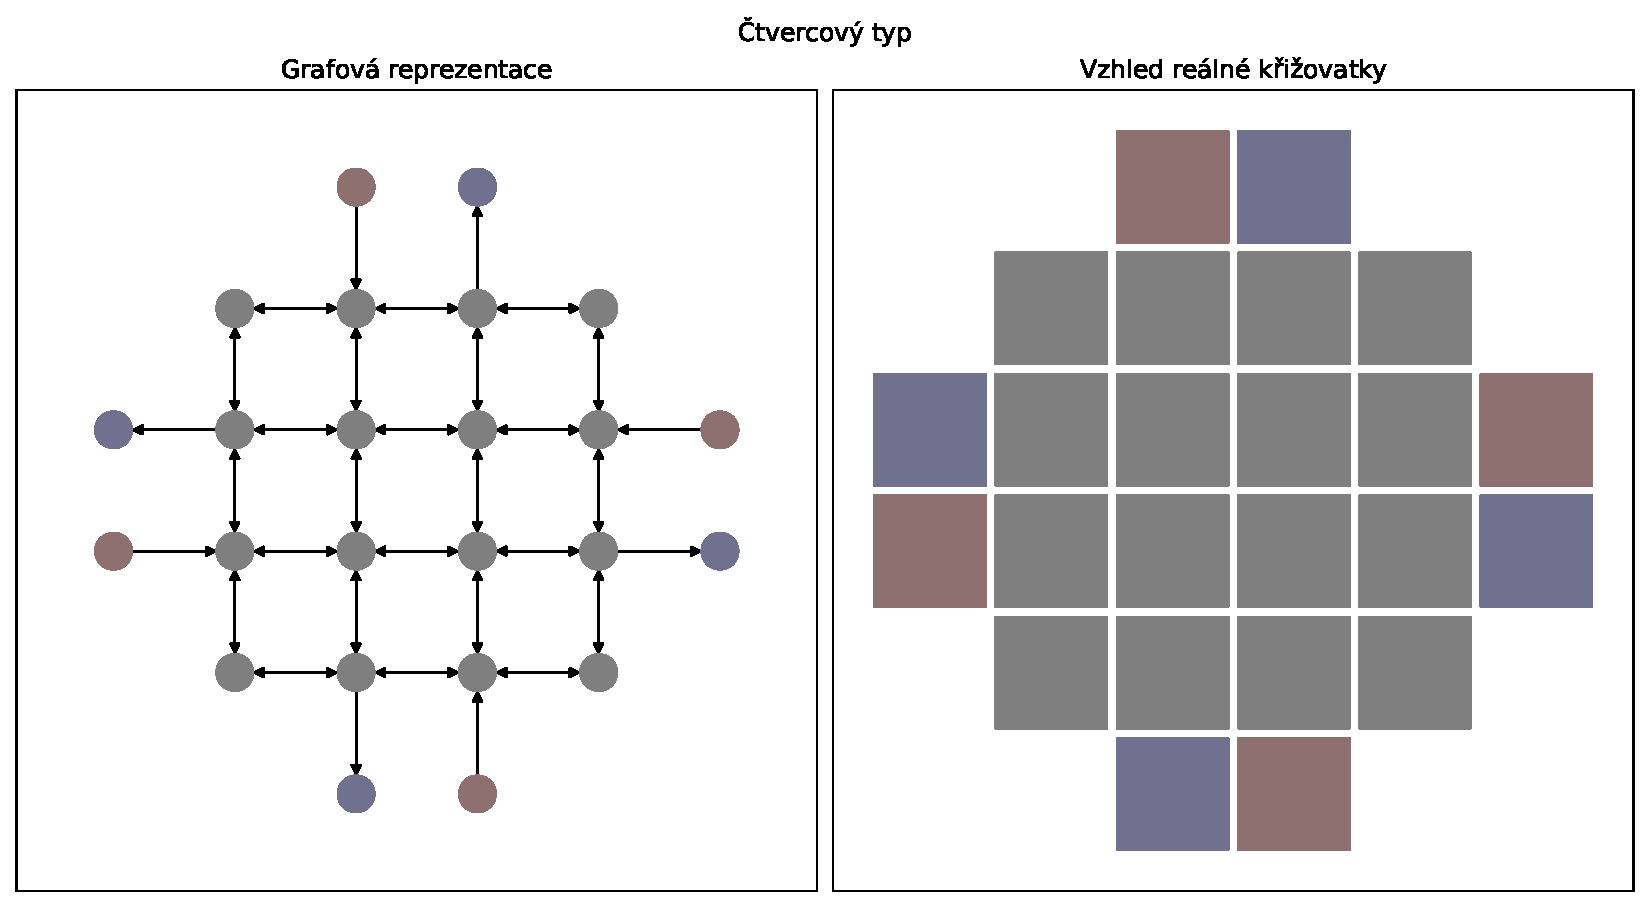
\includegraphics[width=\textwidth]{../img/Square_grid}
%	\caption{Ukázka čtvercového typu křižovatky.}
%	\label{fig:square_type_graph}
%\end{figure}
%
%\subsection{Oktagonální typ}\label{subsec:oktagonalni_typ}
%
%\nameref{subsec:oktagonalni_typ} křižovatky vychází z~\emph{typu čtvercového},
%avšak rozšiřuje tento typ o~možnost diagonální jízdy.
%Tohoto efektu docílí křižovatka přidáním dodatečných vrcholů mezi každé čtvercové bloky dotýkající se rohem.
%Z~vizuálního hlediska se ze~čtvercových bloků stanou oktagonální (osmiúhelníkové),
%odtud plyne samostatný název tohoto typu.
%Tyto bloky mohou mít až~$8$~sousedů.
%Mezi těmito oktagonálními bloky vzniknou nové bloky reprezentující diagonální přejezdy.
%Nově vytvořené bloky mají nanejvýše $4$~sousedy, tvoří tudíž pomyslný čtverec otočený o~$45^{\circ}$.
%Z~vizuálního hlediska byly odebrány rohové bloky.
%
%Vjezdy a výjezdy jsou totožné jako u~\emph{čtvercového typu}.
%
%Granularita, vjezdy a výjezdy mají stejný význam jako u~čtvercového typu.
%Počet vrcholů u~této křižovatky činí $g^2 - 4 + (g-1)^2 + 4i + 4o = 2g^2 - 2g - 3 + 4(i + o)$,
%kde $g$ je granularita, $i$ počet vjezdů a $o$ počet výjezdů.
%Velikost bloku je vzdálenost mezi dvěma sousedními vrcholy reprezentujícími oktagonální blok.
%Tudíž totožná s~velikostí bloku u~čtvercového typu.
%
%Na~obrázku (Obrázek~\ref{fig:octagonal_type_graph}) je znázorněn příklad oktagonálního typu křižovatky s~granularitou~$4$,
%jedním vjezdem a jedním výjezdem.
%
%Barvy vrcholů a bloků jsou stejné jako u~čtvercového typu, šedou barvou jsou označeny vrcholy značící běžnou plochu křižovatky,
%červeno-šedou barvou označeny vrcholy reprezentující vjezdy a modro-šedé vrcholy reprezentují výjezdy.
%
%\begin{figure}[h]
%	\centering
%	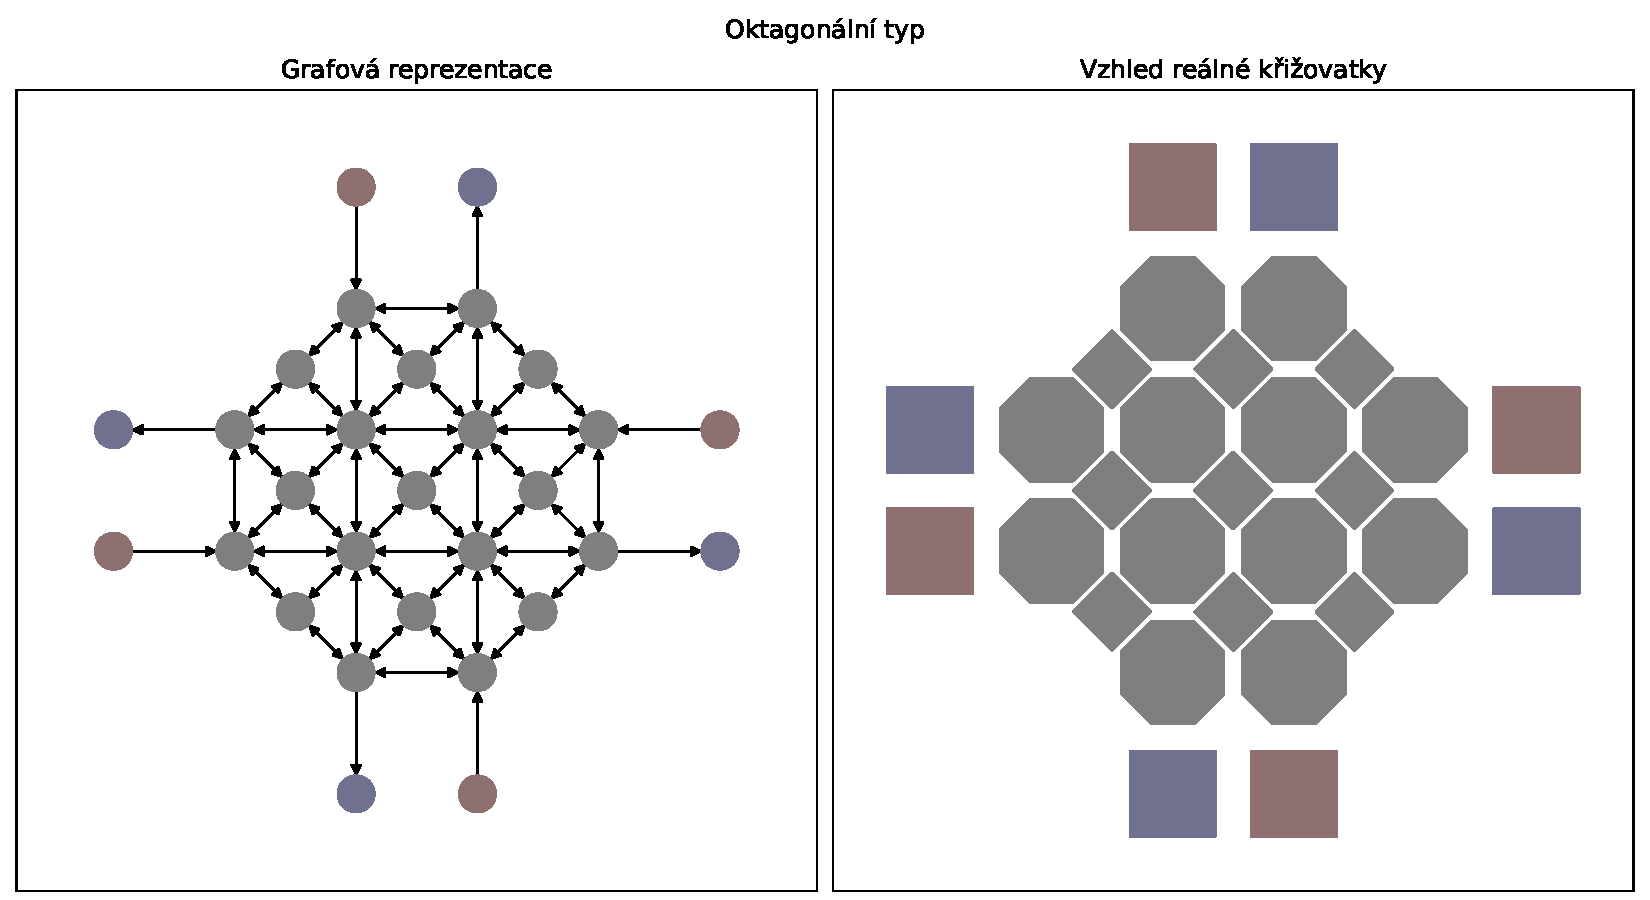
\includegraphics[width=\textwidth]{../img/Octagonal_grid}
%	\caption{Ukázka oktagonálního typu křižovatky.}
%	\label{fig:octagonal_type_graph}
%\end{figure}
%
%\subsection{Hexagonální typ}\label{subsec:hexagonalni_typ}
%
%\nameref{subsec:hexagonalni_typ} je tvořen bloky s~tvary hexagonu (šestiúhelníku).
%Při~převodu křižovatky na graf je každý hexagonální blok nahrazen jedním vrcholem ležícím uprostřed původního bloku.
%Opět hrany grafu vedou mezi bloky se společnou hranou.
%Každý blok má tedy až~$6$~sousedů.
%Tyto bloky tvoří dohromady plochu tvaru velkého hexagonu.
%Díky této reprezentaci má křižovatka tohoto typu $6$~směrů odkud mohou auta přijíždět.
%
%Toto rozdělení sebou nese jednu velkou nevýhodu.
%Pokud chce auto jet rovně skrze křižovatku (do~protilehlého směru), křižovatka mu nemůže nabídnout rovnou cestu.
%
%Granularita u~tohoto typu značí počet bloků na~jedné straně celkové plochy.
%Hodnota je taktéž rovna počtu vrcholů z~kraje křižovatky do~středu.
%Počet vrcholů grafu tedy činí $6 \times g \times (g-1) + 6i + 6o$,
%kde $g$ je granularita, $i$ počet vjezdů a $o$ počet výjezdů.
%Velikost bloku je vzdálenost mezi dvěma sousedními vrcholy.
%
%Na~obrázku (Obrázek~\ref{fig:hexagonal_type_graph}) je znázorněn příklad hexagonálního typu křižovatky s~granularitou~$4$,
%jedním vjezdem a jedním výjezdem.
%
%Barvy vrcholů a bloků jsou opět stejné.
%Šedou barvou jsou označeny vrcholy značící běžnou plochu křižovatky,
%červeno-šedou barvou označeny vrcholy reprezentující vjezdy a modro-šedé vrcholy reprezentují výjezdy.
%
%\begin{figure}[h]
%	\centering
%	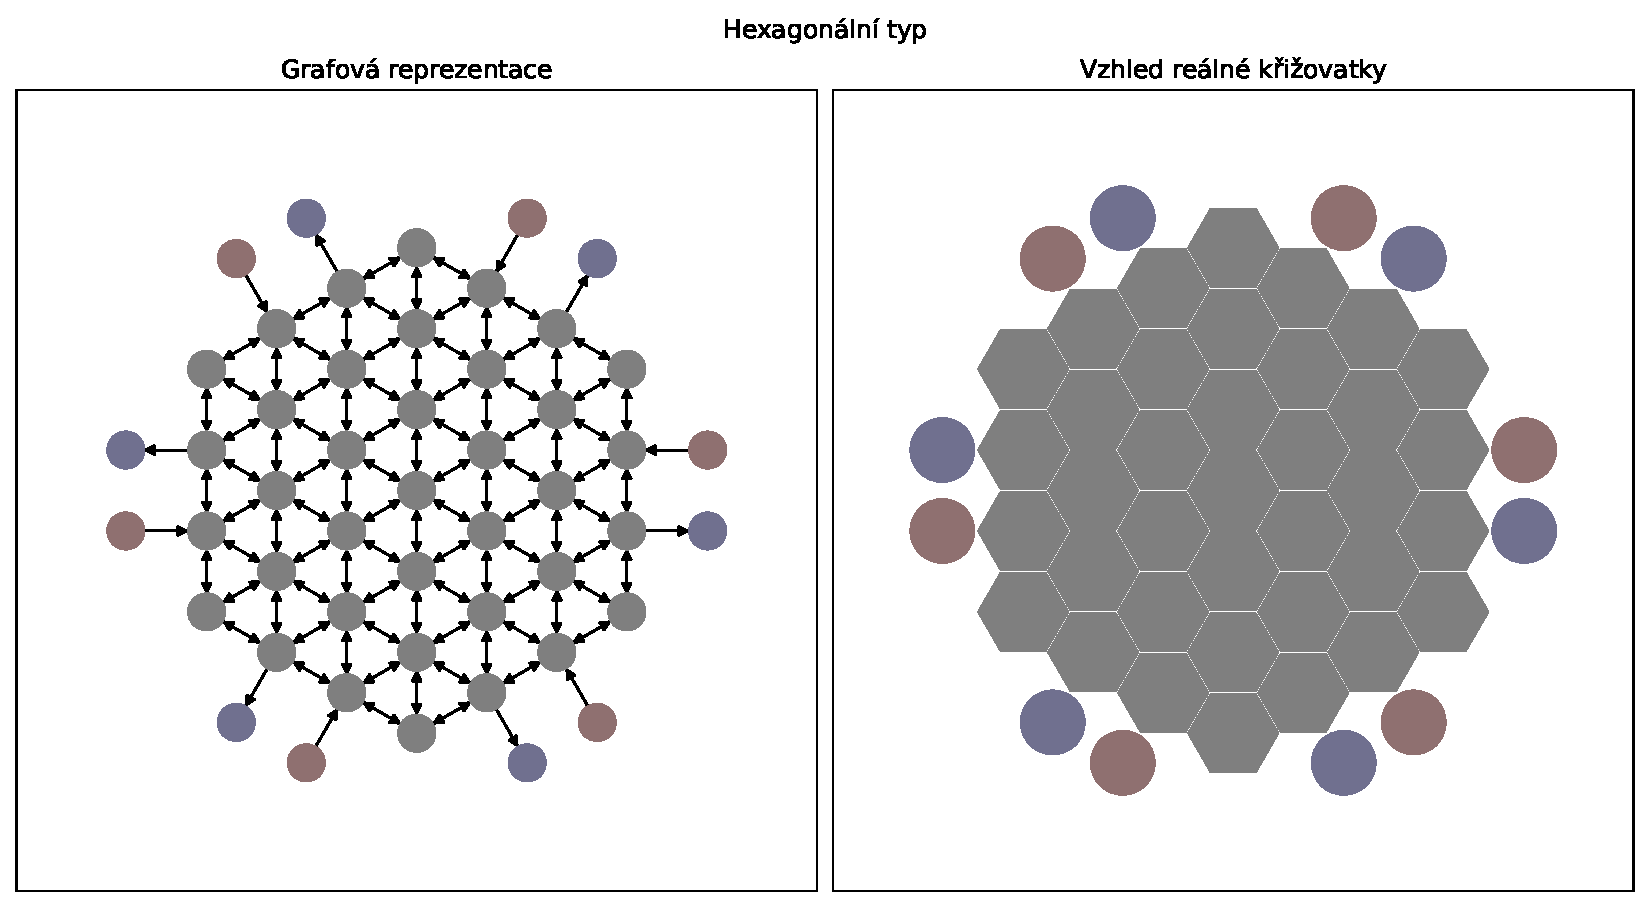
\includegraphics[width=\textwidth]{../img/Hexagonal_grid}
%	\caption{Ukázka hexagonálního typu křižovatky.}
%	\label{fig:hexagonal_type_graph}
%\end{figure}
